\documentclass[tikz, border=10pt]{standalone}
\usetikzlibrary{arrows.meta, bending}

\begin{document}
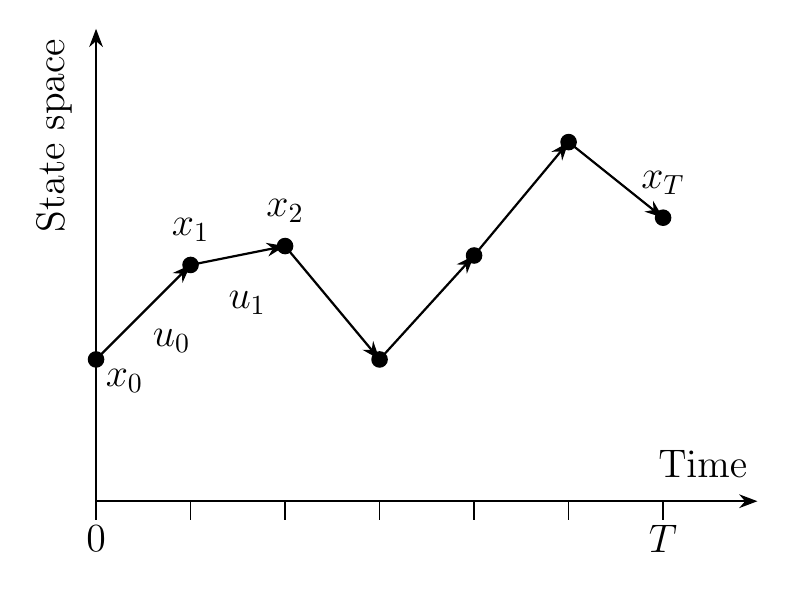
\begin{tikzpicture}[>=Stealth, scale=1.2]

    % Axes
    \draw[->, thick] (0,0) -- (7,0) node[anchor=south east, yshift=5pt] {\Large Time};
    \draw[->, thick] (0,0) -- (0,5) node[rotate=90, anchor=south east, yshift=5pt] {\Large State space};

    % Tick marks on x-axis
    \foreach \x in {0, 1, 2, 3, 4, 5, 6}
        \draw (\x, 0) -- (\x, -0.2);
    
    % Axis labels
    \node at (0, -0.4) {\Large $0$};
    \node at (6, -0.4) {\Large $T$};

    % Define the points for the trajectory
    \coordinate (p0) at (0, 1.5);
    \coordinate (p1) at (1, 2.5);
    \coordinate (p2) at (2, 2.7);
    \coordinate (p3) at (3, 1.5);
    \coordinate (p4) at (4, 2.6);
    \coordinate (p5) at (5, 3.8);
    \coordinate (p6) at (6, 3);

    % Draw the smooth trajectory curve
    %\draw[ultra thick] (p0) to[out=30, in=180] (p1) 
    %                      to[out=0, in=170] (p2) 
    %                      to[out=-60, in=150] (p3) 
    %                      to[out=-30, in=210] (p4) 
    %                      to[out=30, in=160] (p5) 
    %                      to[out=-20, in=150] (p6);

    % Draw the nodes (dots)
    \foreach \p in {p0, p1, p2, p3, p4, p5, p6}
        \fill (\p) circle (2.5pt);

    % State Labels (x_k)
    \node[anchor=north west] at (p0) {\Large $x_0$};
    \node[anchor=south, yshift=5pt] at (p1) {\Large $x_1$};
    \node[anchor=south, yshift=5pt] at (p2) {\Large $x_2$};
    \node[anchor=south, yshift=5pt] at (p6) {\Large $x_T$};

    % Control Vectors (arrows u_k)
    \draw[->, thick] (p0) -- (p1);
    \node at (0.8, 1.7) {\Large $u_0$};
    
    \draw[->, thick] (p1) -- (p2);
    \node at (1.6, 2.1) {\Large $u_1$};

    \draw[->, thick] (p2) -- (p3);
    \draw[->, thick] (p3) -- (p4);
    \draw[->, thick] (p4) -- (p5);
    \draw[->, thick] (p5) -- (p6);



\end{tikzpicture}
\end{document}